\documentclass[11pt,a4paper]{article}
\usepackage[T1]{fontenc}
\usepackage[utf8]{inputenc}
\usepackage[margin=2cm,includefoot,footskip=30pt]{geometry}
\usepackage{amsmath}
\usepackage{amssymb}
\usepackage{helvet}
\usepackage{graphicx}
\usepackage[dvipsnames]{xcolor}
\usepackage{pgfgantt}
\usepackage{parskip}
\usepackage[hidelinks]{hyperref}
\usepackage[polish]{babel}
\usepackage{float}
\usepackage{graphicx,stackengine,scalerel}

\renewcommand{\familydefault}{\sfdefault}
\renewcommand{\arraystretch}{1.5}

\newtheorem{definition}{Definicja}[section]

\def\tang{\ThisStyle{\abovebaseline[0pt]{\scalebox{-1}{$\SavedStyle\perp$}}}}

\begin{document}

    \begin{titlepage}
        \centering
        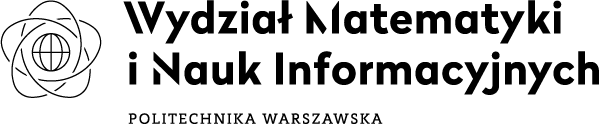
\includegraphics[width=\textwidth]{resources/WMiNI-znak-black.png} \par
        \vspace{3cm}
        {\LARGE Programy działań z efektami domyślnymi \par}
        \vspace{0.5cm}
        {\Large Reprezentacja Wiedzy - projekt \par}
        \vspace{2cm}
        {\large
            Bartosz Borkowicz\\
            Sebastian Konowrocki\\
            Tomasz Laskowski\\
            Piotr Łazarczyk\\
            Jakub Niemyjski\\
            Bartłomiej Pieńkowski\\
            Igor Pieńkowski\\
            Bartłomiej Teodorczuk\\
            Łukasz Wasilewski
        \par}
        \vspace{4cm}
        {\large Wersja 1.0 \par}
        \vspace{0.5cm}
        {\large \today \par}
    \end{titlepage}

    \tableofcontents
    \newpage

    \section{Opis zadania}
    
    Celem projektu jest opracowanie języka akcji oraz odpowiadającego mu języka kwerend dla klasy systemów dynamicznych, która została zdefiniowana poniżej.
    
    Język akcji ma być zaprojektowany dla klasy systemów dynamicznych spełniających następujące warunki:
    \begin{enumerate}
        \item Prawo inercji
        \item Niedeterminizm i sekwencyjność działań
        \item Pełna informacja o wszystkich akcjach i wszystkich skutkach bezpośrednich
        \item Z każdą akcją związany jest
            \begin{itemize}
                \item warunek początkowy (ew. $true$)
                \item efekt akcji
                \item jej wykonawca
            \end{itemize}
        \item Skutki akcji:
            \begin{itemize}
                \item \textit{pewne} - zawsze występują po zakończeniu akcji
                \item \textit{domyślne} - preferowane, zachodzą po zakończeniu akcji, o ile nie jest wiadomym, że nie występują
            \end{itemize}
        \item Efekty akcji zależą od stanu, w którym akcja się zaczyna oraz od jej wykonawcy
        \item W pewnych stanach akcje mogą być niewykonalne przez pewnych (wszystkich) wykonawców
    \end{enumerate}
    
    Język akcji spełniający dane warunki może być odpytywany poprzez odpowiadający mu język kwerend, który zapewnia uzyskanie odpowiedzi prawda ($true$) bądź fałsz ($false$) na następujące pytania:
    \begin{enumerate}
        \item Czy podany program działań jest wykonywalny zawsze/kiedykolwiek?
        \item Czy wykonanie podanego programu działań z dowolnego stanu spełniającego warunek $\pi$ prowadzi zawsze/kiedykolwiek/na ogół do stanu spełniającego warunek celu $\gamma$?
        \item Czy z dowolnego stanu spełniającego warunek $\pi$ cel $\gamma$ jest osiągany zawsze/kiedykolwiek/na ogół?
        \item Czy wskazany wykonawca jest zaangażowany w realizację programu zawsze/kiedykolwiek?
    \end{enumerate}
    
    \subsection{Oznaczenia}
        Na potrzeby uproszczenia definicji oraz opisów w dokumencie wykorzystywane są następujące oznaczenia:
    \begin{itemize}
        \item $A \in \mathcal{A}c$ - akcje
        \item $\omega \in \Omega$ - agenci, w szczególności $\epsilon$ oznacza brak agenta (jakiegokolwiek agenta)
        \item $f \in \mathcal{F}$ - fluenty
        \item $\bar{f}$ - literał odpowiadający $f$, czyli $f$ lub $\neg f$
        \item $\alpha, \pi \in Forms(\mathcal{F})$ - formuły
        \item $\sigma \in \Sigma$ - stany
    \end{itemize}
   
    Formułą nazywamy dowolne połączenie fluentów:
    
    $Forms(\mathcal{F}) \ni \alpha = f~|~\neg \alpha~|~\alpha_1 \wedge \alpha_2~|~\alpha_1 \vee \alpha_2~|~\alpha_1 \Rightarrow \alpha_2~|~\alpha_1 \Leftrightarrow \alpha_2$
    
    Dodatkowo istnieją specjalne formuły:
    \begin{itemize}
        \item $\tang$ oznaczający zawsze prawdę ($true$)
        \item $\perp$ oznaczający zawsze fałsz ($false$)
    \end{itemize}

    \section{Język akcji}
    \begin{definition}[Język $\mathcal{ADA}$]
        Język $\mathcal{ADA}$ jest językiem spełniającym założenia podane w opisie zadania. W poniższych sekcjach zostanie zdefiniowana jego sygnatura, syntaktyka oraz semantyka.
    \end{definition}

    \begin{definition}[Sygnatura]
        Sygnaturą języka $\mathcal{ADA}$ nazywamy parę $\Upsilon=(\mathcal{F},\mathcal{A}c)$, gdzie:
        \begin{itemize}
            \item $\mathcal{F}$ jest zbiorem fluentów
            \item $\mathcal{A}c$ jest zbiorem akcji
        \end{itemize}
    \end{definition}
    
    \subsection{Syntaktyka}
    
    Identyfikatorem jest nazwa akcji, agenta lub fluentu. Identyfikator składa się z ciągu dużych i małych liter alfabetu łacińskiego, cyfr oraz znaku podkreślenia (\_). Dodatkowo identyfikator nie może być żadnym ze słów kluczowych: \textbf{initially}, \textbf{always}, \textbf{observable}, \textbf{after}, \textbf{when}, \textbf{causes}, \textbf{impossible}, \textbf{typically}, \textbf{noninertial}, \textbf{if}, \textbf{not}, \textbf{and}, \textbf{or}, \textbf{then}, \textbf{iff}, \textbf{true}, \textbf{false}. W przypadku identyfikatorów wielkość liter ma znaczenie, to znaczy przykładowo akcje \textit{shoot} i \textit{Shoot} są dwiema różnymi akcjami.

    \subsubsection{Formuły}
    
    Poszczególnym operacjom z konstrukcji formuł odpowiadają następujące zapisy:
    \begin{itemize}
        \item $f \rightarrow identyfikator$ - nazwa fluentu, będąca identyfikatorem zgodnym z opisem powyżej,
        \item $\neg \alpha \rightarrow \mathbf{not}~\alpha$ - negacja logiczna formuły $\alpha$,
        \item $\alpha_1 \wedge \alpha_2 \rightarrow \alpha_1~\mathbf{and}~\alpha_2$ - koniunkcja logiczna formuł $\alpha_1$ i $\alpha_2$,
        \item $\alpha_1 \vee \alpha_2 \rightarrow \alpha_1~\mathbf{or}~\alpha_2$ - alternatywa logiczna formuł $\alpha_1$ i $\alpha_2$,
        \item $\alpha_1 \Rightarrow \alpha_2 \rightarrow \alpha_1~\mathbf{then}~\alpha_2$ - implikacja logiczna formuły $\alpha_1$ w $\alpha_2$,
        \item $\alpha_1 \Leftrightarrow \alpha_2 \rightarrow \alpha_1~\mathbf{iff}~\alpha_2$ - równoważność logiczna (\textit{if and only if}) formuł $\alpha_1$ i $\alpha_2$,
        \item $\tang \rightarrow \mathbf{true}$ - oznacza zawsze prawdę,
        \item $\perp \rightarrow \mathbf{false}$ - oznacza zawsze fałsz.
    \end{itemize}
    
    Dla wyżej wymienionych operacji została zdefiniowana następująca kolejność działań:
    \begin{enumerate}
        \item $\mathbf{not}$
        \item $\mathbf{and}$, $\mathbf{or}$
        \item $\mathbf{then}$
        \item $\mathbf{iff}$
    \end{enumerate}
   
    Nawiasy okrągłe \textit{()} mogą być użyte w celu grupowania wyrażeń oraz zmiany kolejności wykonywania działań matematycznych.
    
    \subsubsection{Instrukcja wartości}
    
    \begin{center}
        $\alpha~\mathbf{after}~\omega_1~A_1,...,\omega_n~A_n$
        \\gdzie $n \geq 1$
    \end{center}
    Formuła $\alpha$ jest \textbf{zawsze} prawdziwa po wykonaniu sekwencji akcji $A_1$ przez agenta $\omega_1$, $...$, $A_n$ przez agenta $\omega_n$. Podanie agenta wykonującego akcję nie jest wymagane. Jeżeli agent nie zostanie podany, wtedy akcja jest wykonywana przez kogokolwiek.
    
    \begin{center}
            $\mathbf{initially}~\alpha$
    \end{center}    
        Jeżeli dla powyższej instrukcji $n=0$, to musimy użyć skróconego zapisu. Oznacza on, że formuła $\alpha$ jest spełniona dla stanu początkowego.
                
    \begin{center}    
        $\mathbf{observable}~\alpha~\mathbf{after}~\omega_1~A_1,...,\omega_n~A_n$
        \\gdzie $n \geq 1$
    \end{center}
    Formuła $\alpha$ jest \textbf{czasem} prawdziwa po wykonaniu sekwencji akcji $A_1$ przez agenta $\omega_1$, $...$, $A_n$ przez agenta $\omega_n$. Podanie agenta wykonującego akcję nie jest wymagane. Jeżeli agent nie zostanie podany, wtedy akcja jest wykonywana przez kogokolwiek.
    
    \subsubsection{Instrukcja efektu}
    
    \begin{center}
        $\mathbf{when}~\omega_1~\mathbf{or}~...~\mathbf{or}~\omega_n~A~\mathbf{causes}~\alpha~\mathbf{if}~\pi$
        \\gdzie $n \geq 1$
    \end{center}
    Jeżeli akcja $A$ jest wywołana przez któregokolwiek z agentów $\omega_1, ..., \omega_n$ w stanie, który spełnia formułę $\pi$, stan wynikowy spełnia formułę $\alpha$.
    
    \begin{center}
        $\mathbf{when}~\omega_1~\mathbf{or}~...~\mathbf{or}~\omega_n~A~\mathbf{causes}~\alpha$
        \\gdzie $n \geq 1$
    \end{center}
    Zapis równoważny z powyższym, jeżeli $\pi \equiv \tang$. Jeżeli akcja $A$ jest wywołana przez któregokolwiek z agentów $\omega_1, ..., \omega_n$, stan wynikowy spełnia formułę $\alpha$.
    
    \begin{center}
        $A~\mathbf{causes}~\alpha~\mathbf{if}~\pi$    
    \end{center}
    Jeżeli akcja $A$ jest wywołana przez dowolnego agenta w stanie, który spełnia formułę $\pi$, stan wynikowy spełnia formułę $\alpha$. Jest to zapis pierwszej instrukcji, jeżeli akcja jest wywoływana przez dowolnego agenta.
    
    \begin{center}
        $A~\mathbf{causes}~\alpha$
    \end{center}
    Zapis równoważny z powyższym, jeżeli $\pi \equiv \tang$. Jeżeli akcja $A$ jest wywołana, stan wynikowy spełnia formułę $\alpha$.
    
    \begin{center}
        $\mathbf{impossible}~\omega_1~\mathbf{or}~...~\mathbf{or}~\omega_n~A~\mathbf{if}~\pi$
        \\gdzie $n \geq 1$
    \end{center}
    Zapis równoważny z pierwszym, jeżeli $\alpha \equiv \perp$. Akcja $A$ nie jest wykonywalna przez żadnego z agentów $\omega_1, ..., \omega_n$, w stanie, który spełnia formułę $\alpha$. 
    
    \begin{center}
        $\mathbf{impossible}~\omega_1~\mathbf{or}~...~\mathbf{or}~\omega_n~A$
        \\gdzie $n \geq 1$
    \end{center}
    Zapis równoważny z powyższym, jeżeli $\pi \equiv \tang$. Akcja $A$ nie jest wykonywalna przez żadnego z agentów $\omega_1, ..., \omega_n$.
    
    \begin{center}
        $\mathbf{impossible}~A~\mathbf{if}~\pi$
    \end{center}
    Akcja $A$ nie jest wykonywalna przez żadnego agenta w stanie, który spełnia formułę $\alpha$.
    
    \begin{center}
        $\mathbf{when}~\omega_1~\mathbf{or}~...~\mathbf{or}~\omega_n~A~\mathbf{typically~causes}~\alpha~\mathbf{if}~\pi$
        \\gdzie $n \geq 1$
    \end{center}
    Jeżeli akcja $A$ jest wywołana przez któregokolwiek z agentów $\omega_1, ..., \omega_n$ w stanie, który spełnia formułę $\pi$, stan wynikowy z reguły powinien spełniać formułę $\alpha$. Efekt $\alpha$ jest \textbf{preferowany} w odróżnieniu do efektów niedeterministycznych, gdzie żaden wynik nie jest preferowany.
    
    \begin{center}
        $\mathbf{when}~\omega_1~\mathbf{or}~...~\mathbf{or}~\omega_n~A~\mathbf{typically~causes}~\alpha$
        \\gdzie $n \geq 1$
    \end{center}
    Zapis równoważny z powyższym, jeżeli $\pi \equiv \tang$. Jeżeli akcja $A$ jest wywołana przez któregokolwiek z agentów $\omega_1, ..., \omega_n$, stan wynikowy z reguły powinien spełniać formułę $\alpha$.
    
    \begin{center}
        $A~\mathbf{typically~causes}~\alpha~\mathbf{if}~\pi$    
    \end{center}
    Jeżeli akcja $A$ jest wywołana przez dowolnego agenta w stanie, który spełnia formułę $\pi$, stan wynikowy powinien spełniać formułę $\alpha$.
    
    \begin{center}
        $A~\mathbf{typically~causes}~\alpha$
    \end{center}
    Zapis równoważny z powyższym, jeżeli $\pi \equiv \tang$. Jeżeli akcja $A$ jest wywołana, stan wynikowy powinien spełniać formułę $\alpha$.
    
    \subsubsection{Instrukcja uwolnienia}
    
    \begin{center}
        $\mathbf{when}~\omega_1~\mathbf{or}~...~\mathbf{or}~\omega_n~A~\mathbf{releases}~\bar{f}~\mathbf{if}~\pi$
    \end{center}
    Wykonanie akcji $A$ przez któregokolwiek agentów $\omega_1, ..., \omega_n$ w stanie, który spełnia warunek $\pi$ \textbf{może}, ale \textbf{nie musi} zmienić wartość inercyjnego fluentu $f$.
    
    \begin{center}
        $\mathbf{when}~\omega_1~\mathbf{or}~...~\mathbf{or}~\omega_n~A~\mathbf{releases}~\bar{f}$
    \end{center}
    Zapis równoważny z powyższym, jeżeli $\pi \equiv \tang$. Wykonanie akcji $A$ któregokolwiek agentów $\omega_1, ..., \omega_n$ \textbf{może}, ale \textbf{nie musi} zmienić wartość inercyjnego fluentu $f$.
    
    \begin{center}
        $A~\mathbf{releases}~\bar{f}~\mathbf{if}~\pi$
    \end{center}
    Wykonanie akcji $A$ przez dowolnego agenta w stanie, który spełnia warunek $\pi$ \textbf{może}, ale \textbf{nie musi} zmienić wartość inercyjnego fluentu $f$. Jest to zapis pierwszej instrukcji, jeżeli akcja jest wywoływana przez dowolnego agenta.
    
    \begin{center}
        $A~\mathbf{releases}~\bar{f}$
    \end{center}
    Zapis równoważny z powyższym, jeżeli $\pi \equiv \tang$. Wykonanie akcji $A$ \textbf{może}, ale \textbf{nie musi} zmienić wartość inercyjnego fluentu $f$.
    
    \subsubsection{Instrukcja ograniczenia}    
   
    \begin{center}
        $\mathbf{always}~\alpha$
    \end{center}
    Każdy stan musi spełniać formułę $\alpha$.
    
    \subsubsection{Instrukcja opisu fluentu}
    \begin{center}
        $\mathbf{noninertial}~f$
    \end{center}
    Oznaczenia fluentu $f$ jako nieinercjalnego.
    
    \subsection{Semantyka}
    
    \begin{definition}[Stan]
    Stanem nazywamy funkcję $\sigma: \mathcal{F} \rightarrow \{\tang, \perp\}$.
    Jeżeli $f \in \mathcal{F}$ i $\sigma(f)=\tang$ to zapisujemy $\sigma \models f$.
    Jeżeli $\alpha \in Forms(\mathcal{F})$ i formuła $\alpha$ jest prawdziwa w stanie $\sigma$ ($\sigma$ jest modelem $\alpha$), to zapisujemy $\sigma \models \alpha$.
    \end{definition}
    
    \begin{definition}[Dziedzina akcji]
    Dziedziną akcji $D$ nazywamy dowolny nie pusty zbiór instrukcji.
    \end{definition}
    
    \begin{definition}[Semantyczna struktura interpretacyjna języka $\mathcal{ADA}$]
    Semantyczną strukturą interpretacyjną języka $\mathcal{ADA}$ nazywamy czwórkę $S=(\Sigma, \sigma_0, ResAb, ResN)$, gdzie:
    \begin{itemize}
        \item $\Sigma$ jest zbiorem stanów
        \item $\sigma_0 \in \Sigma$ jest stanem początkowym
        \item $ResAb: \mathcal{A}c \times \Omega \times \Sigma \rightarrow \Sigma^2$ jest nietypową funkcją przejścia
        \item $ResN: \mathcal{A}c \times \Omega \times \Sigma \rightarrow \Sigma^2$ jest typową funkcją przejścia
    \end{itemize}
    \end{definition}
    
    Niech $D$ będzie dziedziną akcji języka $\mathcal{ADA}$ i niech $S=(\Sigma, \sigma_0, ResAb, ResN)$ będzie jego strukturą. Stan $\sigma$ jest stanem dziedziny $D$ wtedy i tylko wtedy, gdy dla każdej instrukcji ograniczenia typu $\mathbf{always}~\alpha$ zachodzi $\sigma \models \alpha$ w danej dziedzinie $D$.
    
    Niech $Res = ResAb \cup ResN$, $\Psi_S: (\mathcal{A}c \times (\Omega \cup \{ \epsilon \}))^* \times \Sigma \rightarrow \Sigma^2$ będzie mapowaniem takim, że:
    \begin{itemize}
        \item $\Psi_S(\epsilon, \sigma) = \sigma$
        \item jeśli $\Psi_s(((A_1, \omega_1), ..., (A_n, \omega_n), \sigma)$ jest zdefiniowany, to    
    \[
    \Psi_S(((A_1, \omega_1), ..., (A_n, \omega_n), \sigma) \in \left \{
        \begin{array}{ll}
             \bigcup\limits_{\omega \in \Omega} Res((A_n, \omega), \Psi_S((A_1, \omega_1), ..., (A_{1-n}, \omega_{1-n})),~jesli~\omega_n = \epsilon\\
             Res((A_n, \omega_n), \Psi_S((A_1, \omega_1), ..., (A_{1-n}, \omega_{1-n})),~w~p.p.
         \end{array}
     \right.
    \]
    \end{itemize}
    
    Instrukcja wartości typu $(\mathbf{observable})~\alpha~\mathbf{after}~\omega_1~A_1,...,\omega_n~A_n$ jest prawdziwa w $S$ wtedy i tylko wtedy, gdy dla (jakiegokolwiek) \textbf{każdego} mapowania $\Psi_S$
    \begin{itemize}
        \item $\Psi_s(((A_1, \omega_1), ..., (A_n, \omega_n), \sigma)$ jest zdefiniowane oraz 
        \item $\Psi_s(((A_1, \omega_1), ..., (A_n, \omega_n), \sigma) \models \alpha$
    \end{itemize}
    
    Wprowadźmy następujące oznaczenia:
    \begin{itemize}
        \item $New: \mathcal{A}c \times \Omega \times \Sigma \times \Sigma \rightarrow \bar{\mathcal{F}}^2$ jest funkcją, która przypisuje każdej akcji $A \in \mathcal{A}c$, każdemu agentowi $\omega \in \Omega$ i wszystkim $\sigma, \sigma' \in \Sigma$ zbiór literałów $\bar{f}$ takich, że:
        \begin{itemize}
            \item $\sigma' \models \bar{f}$
            \item $f$ jest inercjalny oraz $\sigma \models f \neq \sigma' \models f$ lub\\
            dla jakiejś instrukcji prawdziwe jest $(\mathbf{when}~\omega~A~\mathbf{releases}~f~\mathbf{if}~\pi) \in D \vee (A~\mathbf{releases}~f~\mathbf{if}~\pi) \wedge \sigma \models \pi$
        \end{itemize}
        
        \item $Res_0: \mathcal{A}c \times \Omega \times \Sigma \rightarrow \Sigma^2$ jest funkcją, która dla każdej akcji $A \in \mathcal{A}c$, każdego stanu $\sigma \in \Sigma$ i każdego agenta $\omega \in \Omega$ jest zbiorem wszystkich stanów $\sigma' \in \Sigma$ takich, że:\\
        $(\mathbf{when}~\omega~A~\mathbf{causes}~\alpha~\mathbf{if}~\pi) \in D \vee (A~\mathbf{causes}~\alpha~\mathbf{if}~\pi) \in D \wedge \sigma \models \pi \Rightarrow \sigma' \models \alpha$

        \item $Res^-: \mathcal{A}c \times \Omega \times \Sigma \rightarrow \Sigma^2$ jest funkcją, która dla każdej akcji $A \in \mathcal{A}c$, każdego stanu $\sigma \in \Sigma$ i każdego agenta $\omega \in \Omega$ jest zbiorem wszystkich stanów $\sigma' \in \Sigma$ takich, że zbiory $New(A, \omega, \sigma, \sigma')$ są minimalne.
        
        \item $Res_0^+: \mathcal{A}c \times \Omega \times \Sigma \rightarrow \Sigma^2$ jest funkcją, która dla każdej akcji $A \in \mathcal{A}c$, każdego stanu $\sigma \in \Sigma$ i każdego agenta $\omega \in \Omega$ jest zbiorem wszystkich stanów $\sigma' \in \Sigma$ takich, że:\\
        $(\mathbf{when}~\omega~A~\mathbf{typically~causes}~\alpha~\mathbf{if}~\pi) \in D \vee (A~\mathbf{typically~causes}~\alpha~\mathbf{if}~\pi) \in D \wedge \sigma \models \pi \Rightarrow \sigma' \models \alpha$
    \end{itemize}
    
    \begin{definition}[Model]
    Niech $D$ będzie dziedziną akcji języka $\mathcal{ADA}$. Struktura $S=(\Sigma, \sigma_0, ResAb, ResN)$ jest modelem $D$ wtedy i tylko wtedy, gdy:
    \begin{itemize}
        \item $\Sigma$ jest zbiorem wszystkich stanów dziedziny $D$
        \item wszystkie instrukcje wartości w $D$ są prawdziwe w $S$
        \item dla każdej akcji $A \in \mathcal{A}c$, każdego stanu $\sigma \in \Sigma$ i każdego agenta $\omega \in \Omega$
        \\$ResN(A,\omega,\sigma)=\{\sigma' \in Res_0^+(A,\omega,\sigma) \cup Res_0(A,\omega,\sigma):~ New(A,\omega,\sigma,\sigma')~jest~minimalny\}$
        \\$ResAb(A,\omega,\sigma)=Res^-(A,\omega,\sigma) \textbackslash ResN(A,\omega,\sigma)$
    \end{itemize}
    \end{definition}
    
    \begin{definition}[Program działań]
    Programem działań nazywamy ciąg $((A_1, \omega_1),...,(A_n,\omega_n))$, gdzie $A_i$ jest akcją, zaś $\omega_i$ jej wykonawcą lub $\epsilon$ (ktokolwiek). 
    \end{definition}
    
    \section{Język kwerend}
    
    \subsection{Syntaktyka}
    
    \subsection{Semantyka}
    
    \section{Przykłady}    
\end{document}